\begin{figure}
\centering

\begin{subfigure}{0.45\textwidth}
\centering
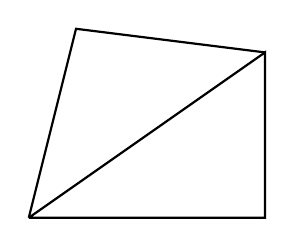
\begin{tikzpicture}[scale=3]
    
    \coordinate (A) at (0,0);
    \coordinate (B) at (1,0);
    \coordinate (C) at (0.2,0.8);
    \coordinate (D) at (1,0.7);
    
    \draw[thick] (A)--(B)--(D)--(A);
    \draw[thick] (A)--(C)--(D);
\end{tikzpicture}
\caption{Non-Delaunay Triangulation}
\end{subfigure}

\hfill

\begin{subfigure}{0.45\textwidth}
\centering
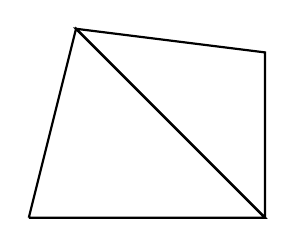
\begin{tikzpicture}[scale=3]    
    % Same points
    \coordinate (A) at (0,0);
    \coordinate (B) at (1,0);
    \coordinate (C) at (0.2,0.8);
    \coordinate (D) at (1,0.7);
    
    % Triangulation (Delaunay: diagonal BC)
    \draw[thick] (A)--(B)--(C)--(A);
    \draw[thick] (B)--(C)--(D)--(B);
\end{tikzpicture}
\caption{Delaunay Triangulation}
\end{subfigure}

\end{figure}